\documentclass[a4paper,11pt]{ltjsarticle}
\usepackage{amsmath, mathtools, mathbbol, amssymb, bm, cancel, fancyhdr, anyfontsize, multirow, wrapfig, graphicx, url, enumitem, ascmac, tikz, tikz-3dplot, makeidx}
\usepackage[luatex]{hyperref}
\usepackage[most]{tcolorbox}
\usepackage{ascolorbox}
\usepackage{stackengine}
\usepackage{cleveref}
\usepackage{appendix, xcolor}
\usepackage{tablefootnote, titlesec}

\hypersetup{
 pdfencoding=auto,
 setpagesize=false,
 bookmarksnumbered=true,
 bookmarksopen=true,
 colorlinks=true,
 linkcolor=blue,
 citecolor=blue,
 urlcolor=blue,
}

\newcommand{\egg}[1]{%
  \raisebox{-3pt}{%
    \begin{tikzpicture}[x=1pt,y=1pt,line width=0.5pt]
      \draw[densely dotted,cap=round] (0,0) ellipse (4.5 and 6);
      \node at (0,0) {\fontfamily{phv}\fontsize{9pt}{0}\selectfont #1\/};
    \end{tikzpicture}%
  }%
}

\crefname{equation}{式}{式}
\crefname{figure}{図}{図}
\crefname{table}{表}{表}

\crefname{section}{}{}
\creflabelformat{section}{#2#1節#3}
\crefname{subsection}{}{}
\creflabelformat{subsection}{#2#1節#3}

\newcommand{\crefpairconjunction}{と}
\newcommand{\crefrangeconjunction}{から}
\newcommand{\crefmiddleconjunction}{，}
\newcommand{\creflastconjunction}{，および}

\makeindex
\numberwithin{equation}{section}
\usepackage[numbers]{natbib}
\usetikzlibrary{arrows, angles, quotes, cd}
\renewcommand{\cite}[1]{\textsuperscript{\citep{#1}}}
\newcommand{\idx}[1]{#1\index{#1}}
\newcommand{\Cancel}[2][black]{{\color{#1}\cancel{\color{black}#2}}}

\pagestyle{fancy}
\rhead{\textbf{\thepage}}
\cfoot{}
\renewcommand{\headrulewidth}{0pt}

\title{\textbf{単位換算の考え方と化学計算}}
\author{寺谷優輝}
\date{\today}

\begin{document}

\maketitle

\begin{abstract}
  本稿では，モル計算と濃度計算を扱う．当然ながら，試薬の調整で必要な知識である．
  微生物を扱う上では，寒天培地をつくる際に\textbf{どのくらいの寒天が必要なのか？}，植物の成分抽出をする上では，\textbf{エタノールの濃度はどのくらいが適切なのか？}などを考える必要がある．
  これらの計算ができない限り，実験系を組むことができず実験のスタートラインに立てない．そのため，まずは計算できるようになることを目的とする．

  化学Chemistryの基本的な考え方は，\textbf{すべての物質は粒で構成されている}ということである．
  その粒の構造や運動を，\textbf{実験的に導かれ}帰納的に体系化されていることを忘れないで欲しい．
\end{abstract}

\tableofcontents

\vspace{12pt}

\begin{center}
  \textbf{\color{blue}青文字}をクリックすると，対応したページに遷移する．\\
  本稿の著作権は，\href{https://creativecommons.org/licenses/by-nc-sa/4.0}{CC BY-NC-SA 4.0}を適応する．
\end{center}

\cleardoublepage

\section{国際単位系International System of units}
\label{sec: si}

\textbf{科学Science}の世界では，測定や計算に\textbf{国際単位系}\cite{units-1}という国際的に統一された単位系を使用する．
この単位系を用いて\textbf{数値と単位の組}でデータを示す．この組のことを\textbf{物理量}Physical quantityという．
7つの\textbf{基本単位}を組み合わせて\textbf{組立単位}にすることで，さまざまな単位を作ることができる．
組立単位を知ることによって，求めたい単位に変える\textbf{単位換算}Unit conversionを行うことができるようになる．

\subsection{基本単位Basic units}
\label{sec: basic units}

基本単位は次の7つである．

\begin{table}[hbtp]
  \caption{基本単位}
  \label{tab: basic units}
  \centering
  \begin{tabular}{rll}
    \hline
    データの種類 & 英語 & 単位 \\
    \hline
    時間 & {\color{cyan}$t$}ime & [s] \\
    距離 & {\color{cyan}$r$}oute & [m] \\
    電流 & {\color{cyan}$I$}ntensity of current & [A] \\
    質量 & {\color{cyan}$m$}ass & [kg] \\
    絶対温度 & {\color{cyan}$T$}emperture & [K] \\
    物質量 & {\color{cyan}$n$}umber & [mol] \\
    光度 & Luminous {\color{cyan}$I$}ntensity & [cd] \\
    \hline
  \end{tabular}
\end{table}

モル計算や濃度計算においては，\textbf{質量}$m$\ [kg]，\textbf{物質量}$n$\ [mol]のみ登場する．
それ以外は参考として載せておくので，眺めてみると良いだろう．

\subsection{物質量Amount of substance}

原子1粒同士を比較しても，非常に小さいため明確に重さの違いは分からない．しかし，何万，何億の粒を集めて比較すると，違いが分かるようになる．
かつては，炭素原子を基準として12\ [g]になるために必要な数である\colorbox{yellow}{$6.022 \times 10^{23}$個(アボカドロ数)}を1\ [mol]としていた．ただし，「炭素」依存での定義であり普遍性に欠ける．

ここでアボガドロ定数$N_A$を$6.022,140,76 \times 10^{23}$\ [/mol]と定義\cite{units-6}することで，単位の大きさを定めた．
簡単に言えば，原子や分子の粒を$N_A$個のことを1\ [mol]と置いた．この考えは，12個を1ダースと置くのと同じである．

物質量以外が何を基準として定義されているのかは，\textbf{\cref{col: basic def}}に記載した．

\subsection{接頭辞Prefix}
\label{sec: prefix}

接頭辞とは，基本単位よりも\textbf{大きい・小さいことを表す指標}のことである．
Si接尾辞では$\times 10^{\pm 30}$まで定まっているが，よく使われる$\times 10^{\pm 12}$までを紹介する．

\begin{table}[htbp]
  \caption{Si接頭辞}
  \label{tab: prefix}
  \centering
  \begin{tabular}{cccccc}
    \hline
    ($+$)接頭辞 & 英語 & 指数乗 & ($-$)接頭辞 & 英語 & 指数乗 \\
    \hline
    T & {\color{cyan}T}era & $\times 10^{12}$ & p & {\color{cyan}p}ico & $\times 10^{-12}$ \\
    G & {\color{cyan}G}iga & $\times 10^{9}$ & n & {\color{cyan}n}ano & $\times 10^{-9}$ \\
    M & {\color{cyan}M}ega & $\times 10^{6}$ & $\mu$ & micro & $\times 10^{-6}$ \\
    k & {\color{cyan}k}ilo & $\times 10^{3}$ & m & {\color{cyan}m}illi & $\times 10^{-3}$ \\
    h & {\color{cyan}h}ecto & $\times 10^{2}$ & c & {\color{cyan}c}enti & $\times 10^{-2}$ \\
    da & {\color{cyan}d}ec{\color{cyan}a} & $\times 10^{1}$ & d & {\color{cyan}d}eci & $\times 10^{-1}$ \\
    \hline
  \end{tabular}
\end{table}

マイナス乗は，プラス乗にすると\textbf{逆数}になる．例えば，$10^{-6}$は$\tfrac{1}{10^6}$である．
また，$10^{-6}$は$\mu$と置き換えられる．この考え方ができるようになると，単位換算が容易になる．

\subsection{単位換算Unit conversion}
\label{sec: convertion}

単位は，\textbf{定義に基づいて}組み立てることで新しい単位ができる．
基本的には，\textbf{同じ意味を持つもの同士を分母と分子に置き}，{\color{cyan}\textbf{約分する}}ことで求めたい単位へと変える．
\cref{eq: uc-1}は，「\textbf{1日は何秒か？}」を求めたものである．恐らく，一度は計算したことがあるだろう．

\begin{equation}
  1\ [\mathrm{day}] = 1\ \Cancel[orange]{[\mathrm{day}]} \times \frac{24\ \Cancel[cyan]{[\mathrm{hr}]}}{1\ \Cancel[orange]{[\mathrm{day}]}} \times \frac{60\ \Cancel[magenta]{[\mathrm{min}]}}{1\ \Cancel[cyan]{[\mathrm{hr}]}} \times \frac{60\ [\mathrm{sec}]}{1\ \Cancel[magenta]{[\mathrm{min}]}} = 86,400\ [\mathrm{sec}] \label{eq: uc-1}
\end{equation}

単位換算を行う上で押さえるポイントは，最初の単位と\textbf{求めたい単位に注目し}
定義として\textbf{どの物理量同士が等しいか}考え約分する必要がある．
今回の場合，1\ [day] と 24\ [hr]は定義より等しいので，分母と分子に置くことで理論上約分でき1と同じ意味となる．

次に，\cref{sec: prefix}の接頭辞を用いた単位換算を扱う．一例として，[mL]を[L]に変える場合を考える．

\begin{equation}
  1,000\ [\mathrm{{\color{cyan}m}L}] = 1,000 \times {\color{cyan}10^{-3}}\ [\mathrm{L}] = 1\ [\mathrm{L}] \label{eq: uc-2}
\end{equation}

[mL]の{\color{cyan}m}は，\cref{tab: prefix}を参照すると指数乗は{\color{cyan}$10^{-3}$}である．
そのため，まず\textbf{接頭辞を指数乗に変える}．そのあと，指数乗を掛けることで単位を換算できる．

当然ながら接頭辞を付けたす場合は，その指数乗の符号を変えたものを掛ければよい．一例として，\cref{eq: uc-2}の逆を考える．

\begin{equation}
  1\ [\mathrm{L}] = 1 \times 10^{{\color{cyan}+}3}\ [\mathrm{{\color{cyan}m}L}] = 1\ [\mathrm{mL}] \label{eq: uc-3}
\end{equation}

\section{組立単位とその意味}

国際単位系を乗除算して表現したい単位を新たに作り出すことができる．この単位のことを\textbf{組立単位}という．
各論的に次に述べる．

\subsection{2乗，3乗のイメージ}

乗算して作り出した単位としては，square meter\ $\mathrm{[m^2]}$，cubic meter\ $\mathrm{[m^3]}$が挙げられる．
meter\ [m]は一次元でありただの\textbf{直線}(\cref{fig: R^1})である．

\begin{figure}[htbp]
  \centering
  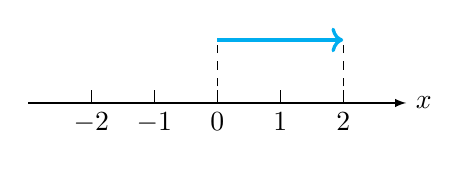
\begin{tikzpicture}[scale=0.8]
    \draw[-latex] (-3,0) -- (3,0) node[right]{$x$};
    \foreach \x in {-2,...,2} \draw (\x,0.2)--(\x,0) node[below] {$\x$};
    \draw[->, very thick, cyan] (0,1) -- (2,1);
    \draw[dashed] (0,0) -- (0,1);
    \draw[dashed] (2,0) -- (2,1);
  \end{tikzpicture}
  \caption{一次元のイメージ}
  \label{fig: R^1}
\end{figure}

そこに[m]を掛けると二次元となり\textbf{平面}(\cref{fig: R^2})である．これは，\textbf{面積}と同じ意味を示している．

\begin{figure}[htbp]
  \centering
  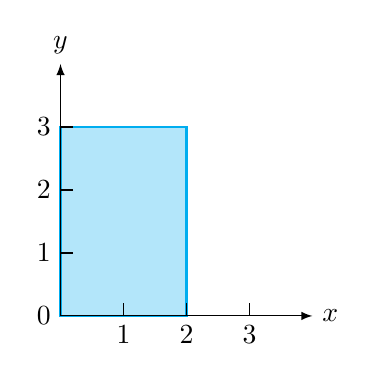
\begin{tikzpicture}[scale=0.8]
    \draw[fill=cyan!30, draw=cyan, thick] (0,0) rectangle (2,3);
    \draw[-latex] (0,0) -- (4,0) node[right]{$x$};
    \foreach \x in {1,...,3} \draw (\x,0.2)--(\x,0) node[below] {$\x$};
    \draw[-latex] (0,0) -- (0,4) node[above]{$y$};
    \foreach \z in {0,...,3} \draw (0.2,\z)--(0,\z) node[left] {$\z$};
  \end{tikzpicture}
  \caption{二次元のイメージ}
  \label{fig: R^2}
\end{figure}

さらに[m]を掛けると三次元となり\textbf{空間}(\cref{fig: R^3})である．これは，\textbf{体積}と同じ意味を示している．

\begin{figure}[htbp]
  \centering
  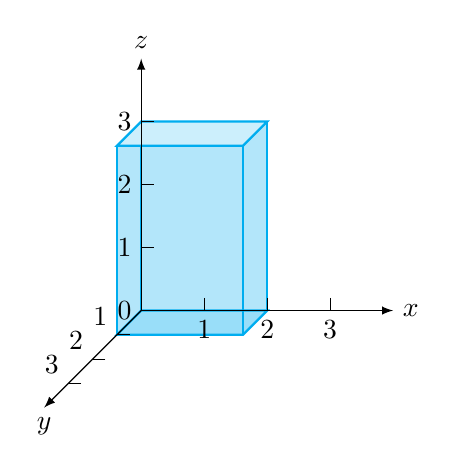
\begin{tikzpicture}[scale=0.8]
    \fill[cyan!30] (0,0,1) -- (2,0,1) -- (2,3,1) -- (0,3,1);
    \fill[cyan!30] (2,0,1) -- (2,0,0) -- (2,3,0) -- (2,3,1);
    \draw[fill=cyan!40, draw=cyan, thick] (2,0,0) -- (2,0,1) -- (0,0,1) -- (0,0,0) --cycle;
    \draw[cyan, thick] (2,0,0) -- (2,3,0);
    \draw[cyan, thick] (2,0,1) -- (2,3,1);
    \draw[cyan, thick] (0,0,1) -- (0,3,1);
    \draw[cyan, thick] (0,0,0) -- (0,3,0);
    \draw[fill=cyan!20, draw=cyan, thick] (2,3,0) -- (2,3,1) -- (0,3,1) -- (0,3,0) --cycle;
    \draw[-latex] (0,0,0) -- (4,0,0) node[right]{$x$};
    \foreach \x in {1,...,3} \draw (\x,0.2,0)--(\x,0,0) node[below] {$\x$};
    \draw[-latex] (0,0,0) -- (0,4,0) node[above]{$z$};
    \foreach \z in {0,...,3} \draw (0.2,\z,0)--(0,\z,0) node[left] {$\z$};
    \draw[-latex] (0,0,0) -- (0,0,4) node[below]{$y$};
    \foreach \y in {1,...,3} \draw (0.2,0,\y)--(0,0,\y) node[above left] {$\y$};    
  \end{tikzpicture}
  \caption{三次元のイメージ}
  \label{fig: R^3}
\end{figure}

\subsection{単位の構成}

単位＊＊\footnote{\textbf{大きさを1}に仕立てた＊＊のこと．}あたりの変化量は，分母に置くこと\footnote{一般に$[/x]$や$[x^{-1}]$と表記されるが，本稿では分かりやすさより$\tfrac{1}{x}$を用いる．}で表現できる．
そのため，一例として\cref{sec: convertion}の\cref{eq: uc-1}の単位は[hr/day]とも表記でき，[/day]は\textbf{1日あたり}という意味となる．

質量は，化学の計算においては\textbf{モル質量}\ [g/mol]の形で計算をする．
モル質量とは，\colorbox{yellow}{1\ [mol]あたりの\textbf{質量}}のことである．各原子ごとに一義の値が経験則から計算されているため，
その値を使えばよい．基本的には周期表に記載されている．日本化学会が公開している周期表を\cref{fig: periodic}に示した．

\begin{figure}[htbp]
  \centering
  \fcolorbox{blue}{white}{
    \href{https://www.chemistry.or.jp/know/atom_2025_ncol.pdf.pdf}{
      \includegraphics[
        page=13,
        angle=-90, 
        width=0.9\textwidth
        ]{atom_2025_ncol.pdf}
    }
  }
  \caption{周期表\cite{periodic-1}}
  \label{fig: periodic}
\end{figure}

\subsection{戸惑いやすいが換算できる単位}

ここから先の内容は，知っているか知らないかの0と1である．そのため，簡単に表にまとめる程度にする．
まずは，一見では換算できなさそうであるが定義上同じものである．

\begin{table}[htbp]
  \caption{戸惑いやすいが換算できる単位}
  \label{tab: unit-1}
  \centering
  \begin{tabular}{cccccc}
    \hline
    体積と質量 & 1\ [cc] &=& 1\ [mL] &=& 1\ [g]\tablefootnote{$4^\circ \mathrm{C}$の水基準である．それ以外では，値が前後することがあるので正確に量り取るときには適さない．} \\
    体積と密度 & 1\ [L] &=& 1\ [dm$^3$] &=& 0.001\ [m$^3$] \\
    モル濃度Molarity & 1\ [M] &=& 1\ [mol/L] \\
    規定度Normality & 1\ [N] &=& 1\ [M] \times\ Eq. &=& 1\ [N]\tablefootnote{モル質量に価数Eq.を乗算したものである．価数は，化学式で表現したときの$\mathrm{H}^+$または$\mathrm{OH}^-$の数である．$\mathrm{Eq.} = 1$のとき，モル濃度と同じである．} \\
    \hline
  \end{tabular}
\end{table}

\subsection{molから換算できる単位}

molを含んだ組立単位を\cref{tab: unit-2}に示す．

\begin{table}[htbp]
  \caption{molから換算できる単位}
  \label{tab: unit-2}
  \centering
  \begin{tabular}{cccccc}
    \hline
    物質量とアボガドロ定数 & 1\ [mol] &=& $6.022 \times 10^{23}$\ [個/mol]\tablefootnote{アボガドロ定数の単位は，一般には「個」を省略して[/mol]を用いる．} \\
    物質量と気体の体積 & 1\ [mol] &=& 22.4\ [L/mol] \\
    物質量と液体の体積 & 1\ [mol] &=& $\tfrac{nm}{\rho}\ [\mathrm{mL/mol}]$\tablefootnote{$n$を物質量，$m$をモル質量，$\rho$を密度とする．} \\
    物質量と固体の体積 & 1\ [mol] &=& $\tfrac{nm}{\rho}\ [\mathrm{cm^3/mol}]$ \\
    \hline
  \end{tabular}
\end{table}

モル質量は大きく3つある．原子量，分子量，式量である．
ただし，この3つは\textbf{無単位量}\footnote{これらは，相対質量として定められている．$^{12}\mathrm{C} = 12$を基準として，\textbf{比の形}で他の原子量を表現する．そのため，単位が約分され無単位量として扱われる．正確な数値は，国際純正・応用化学連合IUPACによって承認されている．}
として扱われているが，相対質量がモル質量と一致するので単位としては[g/mol]で良い．

\begin{table}[htbp]
  \caption{原子量，分子量，式量}
  \label{tab: wt-1}
  \centering
  \begin{tabular}{ccc}
    \hline
    Weight & 略称 & 対象 \\
    \hline
    原子量Atomic Weight & A.W. & 単一原子 \\
    分子量Molecular Weight & M.W. & 共有結合の分子 \\
    式量Formula Weight & F.W. & イオン・塩などの化学式 \\
    \hline
  \end{tabular}
\end{table}

\subsection{百分率は分母に100が隠れてる}

ここからは，濃度の計算を扱う．試薬の調製において，特定のモル濃度や規定度に合わせるときに使う．
質量weight\ [g]と体積volume\ [mL]の違いの組み合わせで，大きく3つの濃度がある．

\begin{table}[htbp]
  \caption{質量\%濃度，質量/体積\%濃度，体積\%濃度}
  \label{tab: con-1}
  \centering
  \begin{tabular}{cccccc}
    \hline
    Concentration & 単位 & 意味 & 単位換算用単位 & 対象 \\
    \hline
    質量百分率 & (w/w)\% & 溶液100\ [g]中の溶質の[g]数 & [g/100g] & 粉末混合 \\
    質量対体積百分率 & (w/v)\% & 溶液100\ [g]中の溶質の[mL]数 & [g/100mL] & 滴定 \\
    体積百分率 & (v/v)\% & 溶液100\ [mL]中の溶質の[L]数 & [mL/100mL] & 溶媒混合 \\
    \hline
  \end{tabular}
\end{table}

またよく使うものを，事前に高濃度で\textbf{ストック溶液stock solution}として用意されている．
これを\textbf{作業溶液working solution}にするためには，希釈dilutionして濃度を下げる操作を行う．

これは単純で，希釈前と希釈後の物質量が\textbf{変化しない}ということさえ押さえておけばよい．
モル\ [mol]はモル濃度\ [mol/L]と体積\ [L]の積で求められるので，\cref{eq: dilution}が成立する．

\begin{equation}
  a\ [\mathrm{mol/L}] \times b\ [\mathrm{L}] = x\ [\mathrm{mol/L}] \times y\ [\mathrm{L}] \label{eq: dilution}
\end{equation}

これで本稿は以上とする．以下に参考文献，付録を追加してある，必要に応じて参考にして欲しい．

\cleardoublepage

\lhead{}
\pagenumbering{alph}
\phantomsection
\addcontentsline{toc}{section}{参考文献}
\bibliographystyle{plain}
\bibliography{ref.bib}

\cleardoublepage
\appendix
\begingroup
\renewcommand{\addcontentsline}[3]{}

\section{ギリシャ文字Greek alphabet}

よく数式の記号でギリシャ文字が用いられるので，知っていると役に立つだろう．

\begin{table}[htbp]
  \caption{ギリシャ文字}
  \label{tab: greek}
  \centering
  \begin{tabular}{rcccrccc}
    \hline
    読み方 &  & 大文字 & 小文字 & 読み方 &  & 大文字 & 小文字 \\
    \hline
    alpha & ｱﾙﾌｧ & A & \alpha & beta & ﾍﾞｰﾀ & B & \beta \\
    gamma & ｶﾞﾝﾏ & \Gamma & \gamma & delta & ﾃﾞﾙﾀ & \Delta & \delta \\
    epsilon & ｲﾌﾟｼﾛﾝ & E & \varepsilon, \epsilon & zeta & ｾﾞｰﾀ & Z & \zeta \\
    eta & ｲｰﾀ & H & \eta & theta & ｼｰﾀ & \Theta & \theta, \vartheta \\
    iota & ｲｵﾀ & I & \iota & kappa & ｶｯﾊﾟ & K & \kappa \\
    lambda & ﾗﾑﾀﾞ & \Lambda &\lambda & mu & ﾐｭｰ & M & \mu \\
    nu & ﾆｭｰ & N & \nu & omicron & ｵﾐｸﾛﾝ & O & $o$ \\
    xi & ｸｼｰ, ｸﾞｻﾞｲ & \Xi & \xi & pi & ﾊﾟｲ & \Pi & \pi, \varpi \\
    pho & ﾛｰ & P & \rho, \varrho & sigma & ｼｸﾞﾏ & \Sigma & \sigma, \varsigma \\
    tau & ﾀｳ & T & \tau & upsilon & ｳﾌﾟｼﾛﾝ & \Upsilon & \upsilon \\
    phi & ﾌｧｲ & \Phi & \phi, \varphi & chi & ｶｲ & X & \chi \\
    psi & ﾌﾟｻｲ & \Psi & \psi & omega & ｵﾒｶﾞ & \Omega & \omega \\
    \hline
  \end{tabular}
\end{table}

\endgroup

\end{document}